\chapter{Wstęp}

\section{Krótki opis procesu}
(uwagi: w dalszej części planuję rozbudować tą sekcję, szkic ten ma na celu po krótce wprowadzić w proces)

Proces badany w pracy to linia montująca płyty drukowane do finalnych produktów.
Sam proces składa się z kilku etapów:
\begin{enumerate}
	\item Pobranie potrzebnych elementów elektronicznych z magazynu.
	\item Uzbrojenie pick\&place w wymagane elementy.
	\item Pobranie gotowych płyt PCB (ang. Printed Circuit Board).
	\item Ręczne nałożenie pasty lutowniczej za pomocą sitodruku
	\item Uruchomienie procesu montażu elementów na maszynie pick\&place
	\item (Opcjonalnie) Umieszczenie ręczne elementów
	\item Przeprowadzenie procesu lutowania w piecu.
	\item (Opcjonalnie) Lutowanie ręczne
	\item (Opcjonalnie) Kontrola gotowej płyty PCB
\end{enumerate}

Cechy procesu:
\begin{itemize}
	\item Wszystkie procedury muszą być wykonane w ustalonej kolejności.
	\item Dla płyt dwustronnych należy powtórzyć sekwencję.
	\item Pick\&place może obsługiwać tylko jedną płytę PCB
	\item Piec lutowniczy może lutować kilka płyt drukowanych (ilość jest zależna od rozmiaru płyt)
	      (uwagi: nie wiem czy to nie skomplikuje zbyt bardzo modelu więc póki co to pominąłem w modelu)
\end{itemize}

\section{Diagram}
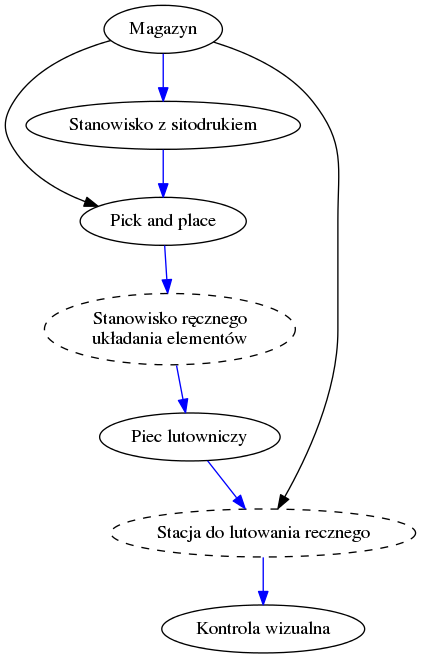
\includegraphics[scale=0.9]{chapters/graph.png}

Niebieskie strzałki wyznaczają ścieżkę krytyczną procesu.
Węzły o krawędziach przerywanych są to operacje zależne od projektu płyty PCB\@.



\section{Model matematyczny}
Problem poruszany w pracy to problem przepływowy (ang. Flow Shop) z przezbrojeniem maszyn.
W procesie jest wykorzystywane 6 stanowisk (maszyn) które składają się na cały proces.
W procesie na dwóch maszynach wykonuję sie przezbrojenie. Jest to stanowisko z sitodrukiem oraz pick\&place.

Zbiór maszyn
\begin{equation}
	M=\lbrace 1,2,\dots,m \rbrace
\end{equation}
gdzie $m$ to liczba maszyn.

Zbiór zadań:
\begin{equation}
	J=\lbrace 1,2,\dots,n \rbrace
\end{equation}
gdzie $n$ to liczba zadań.


Zadanie $j \in J$ jest ciągiem $m$ operacji:
\begin{equation}
	O_{1,j},O_{2,j},\dots,O_{m,j}
\end{equation}

Zmienne w modelu:
\begin{itemize}
	\item $p_{k,j}$ --- czas trwania operacji z zadania $j$ na maszynie $k$
	\item $S_{k,j}$ --- moment rozpoczęcia operacji z zadania $j$ na maszynie $k$
	\item $C_{k,j}$ --- moment zakończenia operacji z zadania $j$ na maszynie $k$
\end{itemize}

Czas przezbrojenia pomiędzy zadaniem $i$ oraz $j$ na $k$-tej maszynie to $s_{i,j}^{k}$ gdzie:
\begin{itemize}
	\item $i \neq j$
	\item  $i,j \in J$
\end{itemize}

Permutacja zadań $\pi = \lbrace \pi(1),\pi(1),\dots,\pi(n) \rbrace$ gdzie $n$ to liczba zadań.

Moment początkowy operacji:
\begin{equation}
	S_{k,\pi(j)}=\max\{C_{k-1,\pi(j)},C_{k,\pi(j-1)}+s^k_{\pi(j-1),\pi(j)}\},
\end{equation}

Obliczenie momentu zakończenia operacji:
\begin{equation}
	C_{k,\pi(j)} = S_{k,\pi(j)} + p_{k,\pi(j)}
\end{equation}

Gdzie $ j \in J$ oraz $k \in M$.

Moment początkowy procesu:
\begin{equation}
	S_{1,\pi(1)}=0
\end{equation}

Moment końcowy procesu:
\begin{equation}
	C_{\max} = 	C_{m,\pi(n)} = S_{m,\pi(n)} + p_{m,\pi(n)}
\end{equation}

W naszym przypadku optymalizacja procesu będzie polegała na wyznaczeniu optymalnej permutacji zadań $\pi^*$
w celu znalezienia minimalnego czasu $C_{\max}$
\begin{equation}
	C_{\max}^{*} = \min\{C_{m,\pi{(n)}^{*}}\}
\end{equation}

\newpage
Z racji że proces jest rzeczywisty to posiada pewne ograniczenia:
\begin{itemize}
	\item musi być zachowany porządek technologiczny operacji,
	      \begin{equation}
	      	O_{1,j} \rightarrow O_{2,j} \rightarrow \dots \rightarrow O_{m,j}
	      \end{equation}
	\item każda operacja może być wykonywana tylko przez jedną maszynę,
	\item żadna maszyna nie może wykonywać więcej jak jednej operacji (uwagi: przypadek kiedy w piecu lutowniczym lutujemy jedną płytę PCB)
	\item wykonywanie żadnej operacji nie może zostać przerwane przed zakończeniem,
	\item momenty rozpoczęcia operacji oraz czas przezbrojenia nie mogą być ujemne
	      \begin{equation}
	      	S_{k,\pi(i)},s^{k}_{\pi(i),\pi(j)} > 0
	      \end{equation}
\end{itemize}
